% ============================================================
\section{Results and Discussion}
\label{sec:results}
% ============================================================

\subsection{Summarization Evaluation (Layer 1)}
Embedding-based TextRank obtains the highest ROUGE scores
(Table~\ref{tab:rouge}). Relative to word-overlap TextRank, ROUGE-1 F1 increases by
approximately 18\% (0.341 to 0.403), and ROUGE-2 F1 increases by approximately
22\% (0.162 to 0.198). The results support semantic rather than lexical edge
weights for the sentence graph.

\begin{table}[!t]
\renewcommand{\arraystretch}{1.2}
\caption{Summarization ROUGE F1 Scores on VietnamNet}
\label{tab:rouge}
\centering
\footnotesize
\begin{tabularx}{\columnwidth}{@{}Xccc@{}}
\toprule
\textbf{Method} & \textbf{ROUGE-1} & \textbf{ROUGE-2} & \textbf{ROUGE-L} \\
\midrule
Lead-K ($k=5$)              & 0.312 & 0.145 & 0.283 \\
Original TextRank           & 0.341 & 0.162 & 0.307 \\
TextRank + TF-IDF           & 0.358 & 0.171 & 0.324 \\
\textbf{TextRank + embedding}   & \textbf{0.403} & \textbf{0.198} & \textbf{0.371} \\
\bottomrule
\end{tabularx}
\end{table}

Sweeping $r\in[0.2,0.6]$ (Table~\ref{tab:retention}), semantic closeness to the title+sapo lead (SemSim) falls while topical coverage (KP-Cov) rises. Both coverage and token cost grow with $r$, so $r=0.4$ is a balanced operating point: it retains sufficient coverage for open-world discovery without inflating the LLM token load.


\begin{table}[!t]
\renewcommand{\arraystretch}{1.2}
\caption{Layer-1 retention sweep; $r{=}0.4$ balances lead similarity and topical coverage}
\label{tab:retention}
\centering
\footnotesize
\begin{tabular*}{\columnwidth}{@{\extracolsep{\fill}}cccc@{}}
\toprule
\shortstack{Retention\\ratio $r$} & \shortstack{Compression\\ratio}
 & \shortstack{Semantic\\similarity $\downarrow$}
 & \shortstack{Keyphrase\\coverage $\uparrow$} \\
\midrule
0.20 & 0.39 & 0.510 & 0.266 \\
0.25 & 0.41 & 0.506 & 0.275 \\
0.30 & 0.45 & 0.501 & 0.287 \\
0.35 & 0.49 & 0.496 & 0.298 \\
\textbf{0.40} & \textbf{0.53} & \textbf{0.490} & \textbf{0.306} \\
0.45 & 0.57 & 0.483 & 0.316 \\
0.50 & 0.61 & 0.477 & 0.324 \\
0.55 & 0.66 & 0.470 & 0.334 \\
0.60 & 0.70 & 0.464 & 0.340 \\
\bottomrule
\end{tabular*}
\end{table}

% \begin{figure}[!t]
% \centering
% 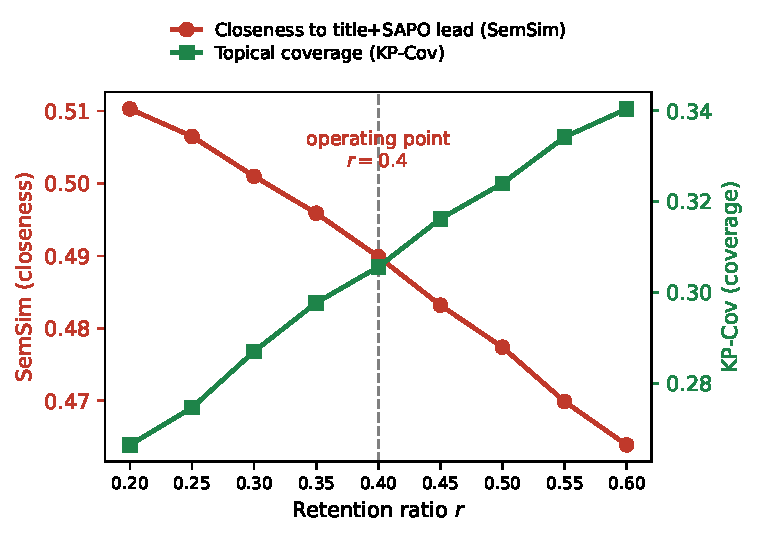
\includegraphics[width=0.92\columnwidth]{figures/retention_balance.pdf}
% \caption{Trade-off over the retention ratio $r$: closeness to the title-and-SAPO lead
% (SemSim, left axis) falls while topical coverage (KP-Cov, right axis) rises. The
% value $r{=}0.4$ is adopted as the operating point.}
% \label{fig:retention}
% \end{figure}

\subsection{Keyphrase-Extraction Evaluation (Layer 2)}
StatLM's KeyBERT leads on every metric (Table~\ref{tab:keyphrase}). The gap between the two KeyBERT variants (F1@10: 30.10 vs. 25.51, about 18\%) confirms the role of \emph{asymmetric embedding} in bridging short keyphrases and long documents. WordAttractionRank leads the graph group (F1@10 = 25.21) but trails KeyBERT because it lacks a redundancy mechanism such as MMR.

\begin{table}[!t]
\renewcommand{\arraystretch}{1.2}
\caption{Keyphrase-Extraction Results on VietnamNet (in \%)}
\label{tab:keyphrase}
\centering
\scriptsize
\setlength{\tabcolsep}{4pt}
\begin{tabular}{@{}lcccccc@{}}
\toprule
\textbf{Method} & \textbf{P@5} & \textbf{R@5} & \textbf{F1@5} & \textbf{P@10} & \textbf{R@10} & \textbf{F1@10} \\
\midrule
RAKE                       & 17.32 & 10.84 & 13.33 & 11.50 & 13.70 & 12.50 \\
YAKE                       & 20.15 & 12.67 & 15.56 & 14.45 & 17.50 & 15.83 \\
TextRank (keywords)        & 19.23 & 12.31 & 15.01 & 13.21 & 16.53 & 14.68 \\
TopicRank                  & 25.02 & 16.45 & 19.85 & 19.34 & 24.52 & 21.62 \\
MultipartiteRank           & 26.83 & 17.67 & 21.31 & 20.47 & 26.26 & 23.01 \\
WordAttractionRank         & 28.49 & 17.43 & 21.63 & 23.16 & 27.66 & 25.21 \\
KeyBERT + sym. emb.        & 28.56 & 17.41 & 21.63 & 23.48 & 27.93 & 25.51 \\
\textbf{KeyBERT (StatLM)}  & \textbf{32.21} & \textbf{21.64} & \textbf{25.89} & \textbf{26.64} & \textbf{34.58} & \textbf{30.10} \\
\bottomrule
\end{tabular}
\end{table}

\subsection{Label-Space and Classification Evaluation (Layer 3)}
Five evaluators independently sorted 72 labels (26 StatLM, 46 X-MLClass-Gemini) into the five groups under a standardized guideline. Fleiss' $\kappa=0.806$ ($\bar P\approx0.866$, $\bar P_e\approx0.307$), an \emph{almost perfect} level according to Landis and Koch~\cite{landis1977}, confirms reliable criteria.

X-MLClass-Gemini produces 18 Entity or Meta/Noise labels, corresponding to a 39.1\% Noise
ratio, and covers 15 of 20 editorial categories with Coarse labels. StatLM produces
one Meta/Noise label, no Entity or Long-tail labels, and covers 19 categories,
yielding a 3.8\% Noise ratio and a 76.9\% Coarse ratio
(Table~\ref{tab:labelspace}). Its five Cross-topic labels reduce fragmentation but
may also obscure distinctions needed downstream. Thus, 19/20 coverage denotes a
compatible coarse label, not exact recovery of the editorial taxonomy.

StatLM obtains $P@1=0.71$ and $P@3=0.84$, compared with 0.49 and 0.63 for X-MLClass-Gemini.
Under the single-label proxy, these measures are top-1 and top-3 accuracy. They do
not capture additional valid document facets that are absent from the reference.
Consequently, the Coarse ratio, Noise ratio, category coverage, and ranking scores
should be interpreted jointly. Optimizing only the Coarse ratio could favor an
over-merged taxonomy, whereas optimizing only coverage could produce redundant or
entity-specific labels. A deployment-oriented evaluation should additionally assess
label stability across batches, hierarchical consistency, and the frequency with
which Cross-topic labels require manual refinement.

\begin{table}[!t]
\renewcommand{\arraystretch}{1.2}
\caption{X-MLClass-Gemini and StatLM Label-Space Quality}
\label{tab:labelspace}
\centering
\footnotesize
\begin{tabular}{@{}lcccc@{}}
\toprule
\multirow{2}{*}{\textbf{Label group}} & \multicolumn{2}{c}{\textbf{X-MLClass-Gemini}} & \multicolumn{2}{c}{\textbf{StatLM}} \\
\cmidrule(lr){2-3}\cmidrule(lr){4-5}
 & \textbf{No.} & \textbf{Ratio} & \textbf{No.} & \textbf{Ratio} \\
\midrule
Coarse      & 15 & 32.6\% & \textbf{20} & \textbf{76.9\%} \\
Long-tail   &  8 & 17.4\% &  0 &  0.0\% \\
Entity      &  6 & 13.0\% &  0 &  0.0\% \\
Meta/Noise  & 12 & 26.1\% &  1 &  3.8\% \\
Cross-topic &  5 & 10.9\% &  5 & 19.2\% \\
\midrule
\textbf{Total} & \textbf{46} & \textbf{100\%} & \textbf{26} & \textbf{100\%} \\
\midrule
Noise ratio                  & \multicolumn{2}{c}{39.1\%} & \multicolumn{2}{c}{\textbf{3.8\%}} \\
Categories covered (Coarse)  & \multicolumn{2}{c}{15/20 (75\%)} & \multicolumn{2}{c}{\textbf{19/20 (95\%)}} \\
\bottomrule
\end{tabular}
\end{table}

\subsection{Performance Evaluation}
On the evaluation platform, StatLM reduces mean processing time from approximately
40 to 10 seconds per document, LLM input from approximately 900 to 30 tokens per document, and API calls from approximately eight to one. These figures correspond to a 75\% time reduction and about 30 times fewer tokens. Absolute latency may differ under other hardware and API conditions.


\subsection{Ablation and Discussion}
Table~\ref{tab:ablation} reports the ablation results for the main
components of StatLM. Each configuration was evaluated on the complete
VietnamNet corpus of 2,000 documents over three independent runs,
while the remaining components, prompts, model settings, and evaluation
procedure were kept unchanged. The reported values are arithmetic means
over the three runs, rounded to the displayed precision.

\begin{table}[!t]
\renewcommand{\arraystretch}{1.25}
\caption{Effect of Each Layer on the Final Label-Space Quality
(L1: ROUGE-1 F1; L2: F1@10; L3: Coarse / Noise / Categories covered).}
\label{tab:ablation}
\centering
\footnotesize
\begin{tabularx}{\columnwidth}{@{}Xcc>{\raggedright\arraybackslash}X@{}}
\toprule
\textbf{Variant} & \textbf{L1} & \textbf{L2} & \textbf{L3 (Coarse/Noise/Cov.)} \\
\midrule
Full StatLM            & 0.403 & 30.10 & 76.9\% / 3.8\% / 19/20 \\
L1 $\to$ orig. TextRank & 0.341 & 28.5 & 68\% / 10\% / 17/20 \\
Drop L1                & --    & 27.0 & 65\% / 15\% / 16/20 \\
L2 $\to$ symmetric      & 0.403 & 25.51 & 70\% / 8\% / 17/20 \\
Drop L2                & 0.403 & --    & 55\% / 20\% / 14/20 \\
\bottomrule
\end{tabularx}
\end{table}

Replacing the embedding-based TextRank in Layer~1 with the original lexical variant reduces ROUGE-1 F1 from 0.403 to 0.341 and degrades the subsequent keyphrase and label-space metrics. Removing Layer~1 further increases the noise-label ratio, indicating that summarization serves not only to reduce document length but also to suppress redundant and peripheral content before keyphrase extraction. The largest degradation occurs when Layer~2 is removed: the coarse-label ratio decreases from 76.9\% to 55.0\%, the noise-label ratio rises from 3.8\% to 20.0\%, and category coverage decreases from 19/20 to 14/20. This result shows that sentence-level summaries alone are insufficient for producing a compact, coarse-grained label space.

Replacing the asymmetric bi-encoder in Layer~2 with a symmetric sentence-embedding model also reduces F1@10 from 30.10 to 25.51 and degrades the final label space. Overall, the results indicate that the two encoder layers make distinct but complementary contributions: Layer~1 improves the semantic concentration of the input, whereas Layer~2 performs topic-oriented condensation and redundancy control before LLM-based generalization. The full configuration therefore provides empirical support for the proposed ``clean first, generalize later'' design.
